\documentclass[a4paper,twoside]{article}
\usepackage[T1]{fontenc}
\usepackage{graphicx}
\usepackage{amsmath,amssymb,amsthm}
\usepackage{booktabs}
\usepackage{array}
\usepackage{pslatex}
\usepackage{apalike}
\usepackage{algorithm2e}
\usepackage[bottom]{footmisc}
\usepackage{url}
\usepackage[hidelinks]{hyperref}
\usepackage{balance}
\usepackage{SCITEPRESS}
\newcommand{\ind}{\mathbf{1}}
\newcommand{\loss}{\mathcal{L}}
\newcommand{\E}{\mathbb{E}}

% Avoid carrying a hyphenated word fragment across a page boundary.
\brokenpenalty=10000
\newcommand{\draftcredit}{\footnote{Drafting assistance: OpenAI Codex \cite{openai2026codex}. See the AI assistance disclosure.}}

\begin{document}
\title{Planning Shared Review for Language Model Workflows with Expiring Intervention Opportunities}
\author{\authorname{Anonymous Submission}}
\keywords{Language Model Agents, Review Scheduling, Decision Support, Tool Workflows, Resource Allocation.}
\abstract{A shared reviewer must decide both which language model errors merit intervention and which can still be addressed in time. We formulate review allocation using finite service duration, public risk estimates and deadline-dependent preventable loss. We implement a transparent queue-order planner and compare it with arrival, urgency, risk and greedy benefit rules. Frozen maintenance experiments show a conditional planning benefit. With two-tick reviews, search reduces mean loss relative to greedy by 1.313 points in a constructed competition workload, while the original workload comparison is close to zero. An adapted retail study uses genuine multistep tool workflows and identical prepared transactions across policies. Its primary comparison is unfavorable to search, with a difference of +0.250 points and a 95\% paired interval of [$-0.333$, $1.000$]. A fresh eight-bundle follow-up gives search 1.667 points more loss than greedy under restricted approval authority, with interval [0.000, 4.667]. Together, the studies separate gains from expiring review opportunities from effects of risk ranking, capacity, objective choice and the reviewer's power to complete a task.}
\onecolumn\maketitle\normalsize\setcounter{footnote}{0}\vfill

\section{INTRODUCTION}
\noindent Several agents may each have a reasonable request for assistance, yet one reviewer cannot address them all before their actions take effect. Reviewing the request with the largest immediate expected benefit may consume the only remaining slot for another useful intervention. Conversely, planning an elaborate review order may accomplish no more than earliest-deadline-first when capacity is sufficient, or may protect a correct transaction while a later mistake expires.\draftcredit

These possibilities arise in workflows where intervention has a service time and a boundary beyond which it cannot undo a consequence. A maintenance correction can stop future downtime without erasing downtime already incurred. A retail approval gate can prevent a mistaken transaction from being posted, but may lack authority to replace it with the intended transaction. The value of a review therefore depends on when it finishes and what the reviewer is allowed to do.

We ask when planning the order of a finite shared review queue improves outcomes over greedy benefit allocation and earliest-deadline-first. We also examine how risk estimates, capacity and the performance objective qualify any benefit. Our evidence combines a controlled civilian maintenance simulation with multistep retail workflows on a local adapted benchmark backend. A follow-up changes reviewer authority and review time separately, preserving preparation and risk estimates.

The contributions are threefold. First, we give an executable formulation that connects public review requests to an application-specific preventable-loss function, while keeping hidden correctness labels outside scheduling. Second, we implement two complementary evaluation protocols: fresh maintenance trajectories with feedback-dependent agent histories, and retail allocation on identical prepared transactions. Third, we provide frozen paired evidence of both planning gains and limits, including an unfavorable practical primary result and a focused operational robustness study. Exact enumeration supplies an interpretable small-queue planner. The contribution concerns the formulation, integration and empirical analysis rather than a new exhaustive scheduling algorithm.

\section{RELATED WORK}
\noindent Help-seeking, communication and constrained deferral address related parts of the oversight problem. KnowNo uses calibrated prediction sets to decide when a language model planner should request help \cite{ren2023knowno}. Its request-admission mechanism and coverage assumptions differ from ordering an already admitted queue. Our uncertainty-first baseline ranks estimated error probability; it does not reproduce KnowNo or provide a conformal guarantee.\draftcredit

Value of Information evaluates clarification by its expected decision utility relative to communication cost \cite{dong2026voi}. We similarly express intervention value through an explicit objective, but allocate a reviewer among competing pending transactions rather than choose a clarification question. One Human, N Agents studies a limited audit budget under miscalibrated and correlated confidence \cite{zavattari2026onehuman}. That work directly establishes shared auditing as prior research. Our focus is finite-duration intervention before a posting or correction cutoff, including the difference between blocking an error and completing a task.

DeCCaF learns expert correctness and uses cost-sensitive constrained allocation across experts \cite{alves2024deccaf}. We retain a single idealized reviewer to isolate sequencing and intervention authority. These are conceptual comparisons of mechanisms, not reproductions of those complete systems. Author-linked implementations of KnowNo, Value of Information and DeCCaF were inspected. No author-linked released implementation for One Human, N Agents was located in the checked paper and project searches.

Classical scheduling already studies deadlines, processing time and weighted consequences. Hariri et al. consider weighted late work, meaning processing performed after a due date \cite{hariri1995latework}. Guo et al. analyze a Pareto tradeoff between weighted tardy-job counts and weighted late work \cite{guo2022pareto}. Our losses differ, but the connection explains why urgency, count objectives and cost objectives can favor different schedules. Exhaustive current-queue search is an established method for a bounded scheduling problem.

The retail substrate is $\tau$-bench, which supplies interactive tasks, domain policies, database tools and annotated final-state validation \cite{yao2024tau}. We reuse its pinned retail implementation while changing the user interaction and adding staging, cutoffs and review. This adaptation makes transaction review testable while retaining genuine retrieval, item selection, payment and mutation semantics.

\section{REVIEW ALLOCATION MODEL}
\noindent A released review request $i$ exposes an arrival time $a_i$, a cutoff $d_i$, a proposed action, review duration $s_i$, public consequence parameters and an estimated initial-error probability $p_i$. The scheduler sees only released requests. It cannot inspect a hidden correct action, a future job or a future model output. A single nonpreemptive reviewer processes one request at a time. Definitive diagnosis becomes available only when that review finishes.\draftcredit

Let $G_i(T)$ be the preventable consequence if request $i$ is initially wrong and an effective review completes at time $T$. The expected benefit is
\begin{equation}
 B_i(T)=p_iG_i(T).
 \label{eq:benefit}
\end{equation}
Eligibility requires release and positive benefit from starting now, $B_i(t+s_i)>0$. A cutoff equality is timely. Consequences incurred before completion remain incurred. The reviewer is perfect in diagnosis throughout these experiments, while its corrective authority is varied explicitly in retail.

\subsection{Policies and Planning}
FCFS selects the earliest eligible arrival. Earliest-deadline-first (EDF) selects the earliest cutoff. Uncertainty-first selects the largest $p_i$. Delay-aware greedy selects the largest $B_i(t+s_i)$. Queue-order search enumerates ordered subsets $\pi$ of the eligible current queue and maximizes
\begin{equation}
 \sum_{k=1}^{|\pi|} B_{\pi_k}\left(t+\sum_{j=1}^{k}s_{\pi_j}\right).
 \label{eq:search}
\end{equation}
It dispatches the first request and replans when free. It does not plan with unreleased arrivals or hidden labels, and it is not a full-horizon optimal-control solution. Ties prefer fewer reviews and then the declared lexicographic arrival, agent and request order. Value sums use stable summation. Historical numerical audits distinguish exactly co-optimal tie differences from positive decision regret.

There are $\sum_{k=0}^{q}q!/(q-k)!$ ordered subsets for $q$ eligible requests. This is 16 at three requests and 1,957 at six. We enumerate them all without queue truncation. Retail additionally includes a no-review control with the same automatic safeguards. Maintenance includes a myopic-benefit baseline; its terminal-only greedy equivalence is checked rather than presented as independent evidence.

\subsection{Pairing and Interpretation}
An exogenous scenario fixes jobs or source cases, arrivals, deadlines and costs. A policy run is not an independent scenario. Maintenance conditions share exogenous streams but receive fresh generations and separate feedback histories. Retail conditions share a saved prepared transaction within a generation replicate because no model generation follows staging. Thus retail isolates allocation on identical inputs, while maintenance measures integrated trajectories that may also differ in model behavior.

For each declared primary comparison, we compute scenario-level paired loss differences and a percentile interval from 2,000 bootstrap resamples. Retail first averages three generation replicates within each source bundle. All conditions for a scenario are resampled together. Other contrasts are secondary, with no multiplicity adjustment. A wide interval spanning zero is uncertainty about the effect, not evidence of equivalence.

\section{CONTROLLED MAINTENANCE STUDY}
\noindent The maintenance environment exposes binary ventilation faults through two independent noisy clues. Faults have equal prior probability, with clue accuracies 0.8 and 0.6. An agent chooses a filter replacement or sensor reset from a public manual. Two fresh model samples are drawn per job. The first action executes; the second supplies agreement information. Review may correct the executed action and provide definitive feedback for later jobs.\draftcredit

An initially wrong action incurs downtime rate $c_i$ until correction or deadline, plus terminal incorrect-closure penalty $K_i$. A timely correction at $T$ prevents
\begin{equation}
 G_i(T)=\ind[T\leq d_i]\{c_i(d_i-T)+K_i\}.
 \label{eq:maintenance}
\end{equation}
The original workload uses three agents, two jobs each and a 12-tick horizon. Releases occur at wave bases 0 and 6 with zero-or-one jitter. Relative windows are drawn from 1, 2 and 5, downtime rates from 0, 1 and 3, and terminal penalties from 0 and 8.

A constructed competition workload releases all three jobs together at 0 and 6. Each wave independently permutes windows 2, 4 and 5 and penalties 4, 8 and 12, with zero downtime. It was motivated by limited competition in earlier development, then evaluated on new frozen scenarios. A larger workload has three or six agents, three jobs each, a 24-tick horizon and waves at 0, 8 and 16 with independent zero-or-one jitter. Windows are 2, 4 and 6, downtime rates 0, 1 and 3, and penalties 0, 4, 8 and 12. Stable per-agent streams pair the first three agents across team sizes. Public assignments are independent of hidden faults.

\subsection{Risk and Frozen Evaluation}
The primary risk estimate is an agreement-bin estimator fit on an earlier development set. Laplace smoothing gives $(e+1)/(n+2)$ for $e$ errors among $n$ jobs; bins with fewer than ten examples use pooled calibration risk. Initial first-action labels are included regardless of review selection. The frozen values are $13/89$ for agreement and pooled $18/98$ for sparse disagreement.

Alternative estimates use pooled risk or a public analytical reference with knowledge of the synthetic observation model. Following agreeing clues has error probability $1/7$; following the stronger disagreeing clue has error probability $3/11$. Choosing the opposite action gives the complementary probability. The reference does not inspect the realized fault. Both samples are retained in every condition. Prediction rescoring uses saved outputs; policy comparisons under alternative risk use actual new trajectories.

The frozen evaluation contains 2,752 episodes. Original and competition workloads each use 64 scenarios and six policies at one- and two-tick reviews. Alternative-risk comparisons use the first 32 scenarios of each workload for greedy and search. Larger-workload comparisons use 32 scenarios with four policies across both team sizes and capacities. A separately declared objective study uses 16 scenarios. The development and evaluation partitions remain separate.

\subsection{Results and Boundary Conditions}
Table~\ref{tab:maintenance} reports central search--greedy contrasts. At two ticks, search gains in constructed competition but has little measured advantage in the original workload. It wins, ties and loses against greedy on 15, 42 and 7 competition scenarios, versus 3, 59 and 2 original scenarios. Search versus EDF in two-tick competition is $-2.5625$ points, with interval [$-4.0000,-1.3125$]. At one tick, search and EDF both attain zero competition loss despite different review sequences on 62 of 64 scenarios.

\begin{table*}[t]
\caption{Frozen maintenance results. Differences are search minus greedy mean loss with 95\% paired scenario-bootstrap intervals. Workload distributions are analyzed separately.}
\label{tab:maintenance}\centering\small
\begin{tabular}{llrrrrl}
\toprule
Workload & Agents / scenarios & Review ticks & Search & Greedy & EDF & Paired difference \\
\midrule
Original & 3 / 64 & 2 & 7.328 & 7.422 & 7.656 & $-0.094\;[-0.563,\;0.344]$ \\
Competition & 3 / 64 & 2 & 1.688 & 3.000 & 4.250 & $-1.313\;[-2.250,-0.438]$ \\
Competition & 3 / 64 & 1 & 0.000 & 0.375 & 0.000 & $-0.375\;[-0.688,-0.125]$ \\
Larger & 6 / 32 & 1 & 16.188 & 22.375 & 23.688 & $-6.188\;[-9.376,-3.281]$ \\
Larger & 6 / 32 & 2 & 36.563 & 36.781 & 46.000 & $-0.219\;[-2.313,\;1.969]$ \\
\bottomrule
\end{tabular}
\end{table*}

The larger workload gives a stronger one-tick planning benefit and a small, uncertain two-tick difference. Reduced capacity does not monotonically increase the value of planning. Some requests are already infeasible when the reviewer becomes free. In the original two-tick search runs, only 32 of 156 dispatches have multiple eligible requests, whereas competition has 224 of 256. Such public contention is a prerequisite for many sequencing effects, but it does not guarantee competing actual errors.

Risk calibration and allocation utility diverge. The frozen estimator predicts roughly 0.15 error while observed errors reach about 0.25--0.32. On two-tick search trajectories, analytical risk improves Brier score from 0.213 to 0.157 in the original workload and from 0.200 to 0.164 in competition. Yet fresh matched-prefix alternative-risk rollouts yield no consistent allocation gain. Better probability scores alone do not establish better counterfactual policy performance.

Weighted cost also differs from task correctness. In the six-agent one-tick workload, search has lower loss than EDF but more incorrect closures. Adding a declared penalty $\lambda$ per incorrect closure to the search objective changes both intervention benefit and eligibility. With $\lambda=8$ rather than zero, original cost increases by 1.75 points [$0.188,3.438$], while incorrect closures decrease by 0.75 [$0.375,1.125$] per scenario. The common augmented objective $\loss+8U$ improves by 4.25 points, where $U$ counts incorrect closures. At two ticks this improvement weakens and the augmented objective is slightly worse. This is a tradeoff between objectives, not a universally superior policy.

\section{ADAPTED RETAIL TRANSACTION STUDY}
\noindent We pin $\tau$-bench retail revision \texttt{59a200c6d575} and retain its policy, tools, task records and final-state validator semantics. Supported families are cancellation, pending-order item modification and delivered-order returns/exchanges. Agents authenticate, retrieve account and order details, inspect available variants, request confirmation and invoke a mutation tool. The tool arguments identify actual local database records. Upstream status, inventory, item compatibility, payment and balance checks remain enabled. Added target-blind guards require ownership, prior retrieval, nonempty transactions and exact-argument confirmation.\draftcredit

A scripted customer exposes the original operational instruction and confirms displayed proposals without independently auditing backend identifiers. Personality directions are removed. The supported cases require one state-changing transaction and no additional textual answer. This bounds the workflow while preserving multiple retrieval and interpretation steps. The experiment is an adapted benchmark study, with no official $\tau$-bench score implied.

\subsection{Intervention Boundary and Objective}
A valid mutation is staged on a copy of the account state. Three independently prepared transactions then enter a simulated processing batch at arrival slots 0, 0 and 1. Relative windows 2, 4 and 5 and processing weights 4, 8 and 12 are separately permuted. At completed review, a perfect corrective reviewer substitutes the annotated transaction and commits it. Otherwise the original proposal posts at cutoff. A posted consequence cannot be erased by a later review. An unstaged preparation has no review request.

The retail loss is
\begin{equation}
 \loss=\sum_i \{4(1-C_i)+W_i M_i\},
 \label{eq:retail}
\end{equation}
where $C_i$ denotes annotated task completion and $M_i$ a wrong committed transaction. $W_i$ is a public processing/rework consequence weight. For corrective review,
\begin{equation}
 G_i^{\mathrm{correct}}(T)=\ind[T\leq d_i](4+W_i).
 \label{eq:correct}
\end{equation}
These are synthetic consequence points and abstract service times. They do not estimate retailer money or human speed.

The boundary is coherent for a service that can gate tool dispatch, but its scope matters. The upstream tools themselves mutate state immediately. Return and exchange tools create requests, not completed physical returns. Platform documentation distinguishes order editing, cancellation and later return processing \cite{shopify2026editing,shopify2026cancel,shopify2026returns}. It supports multiple operational stages, not our numerical deadlines or an assertion that every posted request causes irreversible physical harm. Here irreversibility means that an incurred posting consequence is not refunded within the episode.

The original reviewer can replace the full transaction without another customer conversation. This is stronger than approval. The upstream policy requires confirmation of consequential details, so correcting a previously confirmed wrong proposal is an explicit authority assumption. The follow-up below isolates this assumption. Exact final-state equality is also stricter than some notions of operational equivalence: reason, payment and item-list differences can fail an annotated task even when an order status changes as intended.

\subsection{Development and Pairing}
The original retail study selects 24 development and 96 evaluation cases from training records, with 120 distinct customer accounts. Source-order selection and annotated-transaction checks precede model outputs. The evaluation contains 32 three-case bundles with three fresh preparation replicates, yielding 288 GPU workflows. Six policies and two capacities share each prepared transaction, producing 1,152 paired policy episodes. These are 32 independent source bundles for paired analysis, not 1,152 independent scenarios. Broad templates remain shared and public records may have appeared in model training.

A development-only risk estimator uses public workflow family and a flag for non-high confidence or an earlier automatic rejection. All 64 staged calibration proposals are flagged. The smoothed risks are 0.0400 for cancellation, 0.2917 for modification and 0.4762 for returns/exchanges. Sparse bins use pooled risk 0.2424. Initial labels precede correction and include all staged proposals regardless of review. Eight unstaged development failures remain in outcome reporting but do not have a conditional staged-proposal risk label. No evaluation label updates this estimator.

All application inference uses the same pinned Qwen2.5-7B-Instruct revision in BF16 on one RTX 6000 Ada, with zero CPU model offloading. Temperature is 0.3 and top-$p$ is 1.0. Retail uses one structured sample per tool turn, a 16,384-token server context, at most 15,872 input tokens and 512 output tokens, and a 14-call workflow limit. This differs from maintenance's two action samples per job. Host orchestration, tokenization, scoring and scheduling run on CPU.

\subsection{Original Retail Results}
Of 288 preparations, 233 stage a transaction, 182 are initially correct and 51 stage a wrong valid transaction. Fifty-five never stage. Table~\ref{tab:retail} retains every failure. The primary two-tick search minus greedy difference is $+0.2500$ points, with a 95\% paired interval of [$-0.3333,1.0000$]. Search wins on one bundle, ties on 29 and loses on two. It completes 190 reviews versus greedy's 169, but corrects 40 errors versus 41. The point estimate is unfavorable and does not demonstrate a population disadvantage or advantage.

\begin{table}[t]
\caption{Original retail mean loss and correct tasks. Two-tick correct counts have denominator 288.}
\label{tab:retail}\centering\small
\begin{tabular}{lrrr}
\toprule
Policy & 1 tick & 2 ticks & Correct, 2 ticks \\
\midrule
No review & 8.333 & 8.333 & 182 \\
FCFS & 2.292 & 5.000 & 210 \\
EDF & 2.292 & 4.583 & 215 \\
Uncertainty & 2.292 & 3.458 & 223 \\
Greedy & 2.292 & 3.458 & 223 \\
Search & 2.292 & 3.708 & 222 \\
\bottomrule
\end{tabular}
\end{table}

At one tick every review policy corrects all 51 staged errors, matching a parallel-perfect-review reference. Remaining loss is exactly 55 unstaged failures times four points. Different orders therefore need not change realized loss. Search and greedy sequences differ in 47 of 96 two-tick runs, while only three bundle-mean differences are nonzero. On search's states they choose different heads at 47 of 103 competitive dispatches. Only four two-tick search dispatches contain two initially wrong eligible requests, counted retrospectively with labels excluded from scheduling.

Risk improves aggregate Brier score over pooled calibration risk, 0.15585 versus 0.17153, with AUROC 0.7096. Its family ranking nevertheless reverses between modification and returns/exchanges. Observed modification error is 24/58, above predicted 0.2917, while returns/exchanges have 27/88 errors, below predicted 0.4762. Every staged cancellation is correct. Better aggregate scoring does not ensure the relevant dispatch ranking.

Automatic guards block 778 tool calls, including 338 attempted mutations. Valid semantic errors still include wrong available variants and omitted requested items. Of the 55 unstaged failures, 50 exhaust the step limit, four finish without staging and one exhausts a generation retry. Modification contributes 38 failures. These errors establish a preparation bottleneck outside the transaction reviewer's scope.

\section{OPERATIONAL ROBUSTNESS STUDY}
\noindent A source-based methodological review identified corrective authority, confirmation, family-specific processing stages, review complexity and consequence valuation as unresolved assumptions. It was not independent human expert validation. We froze two one-factor changes, retaining the original condition at both base capacities, the same six policies and the frozen application estimator.\draftcredit

\subsection{Authority and Complexity Changes}
Under restricted authority, a completed review perfectly detects whether the staged proposal is wrong. A correct proposal is approved unchanged. A wrong proposal is blocked, leaving the account unchanged and the service unresolved. It is removed from the queue and cannot post later. Blocking counts neither as task completion nor correction. The preventable loss is therefore
\begin{equation}
 G_i^{\mathrm{block}}(T)=\ind[T\leq d_i]W_i.
 \label{eq:block}
\end{equation}
The missing service benefit is substantive. Since $W_i$ varies, replacing $4+W_i$ by $W_i$ is not a uniform rescaling and can change risk-weighted rankings. Perfect detection remains idealized, and labels are still unavailable before completed review.

The separate complexity condition retains full correction authority and uses
\begin{equation}
 s_i=s+\ind[\text{proposed item-list length}\geq 2],
 \label{eq:complexity}
\end{equation}
where $s$ is one or two ticks. This public proxy captures an additional item-checking burden without fitting review times. A mistaken omission may reduce the apparent complexity, which is retained as a limitation. Arrivals, cutoffs, consequence weights, preparation and risk remain unchanged. We do not evaluate an authority-by-complexity factorial design.

Two outcomes follow mathematically. No-review loss is invariant across variants. Under perfect blocking, every policy's correct-task count equals the initially correct staged count, since neither a wrong nor an unstaged request can be completed by blocking. These invariances are semantic checks rather than empirical discoveries.

\subsection{Fresh Source Cases and Analysis}
We audit all 500 train, 20 dev and 115 test records at the pinned revision, excluding all 120 Stage 5 accounts across source splits. Eligibility retains the original explicit-instruction, supported single-transaction criteria and source-intent consistency checks. Only ten unused eligible modification accounts remain, so a 16-bundle design is infeasible. The declared fallback selects eight globally disjoint bundles from 24 training cases, reserving modification first and then cancellation and returns/exchanges in source order. The source pool is not filtered using model outcomes or expected scheduling gains.

Three fresh replicates yield 72 workflow attempts. The same preparations feed six policies, two base durations and three operational variants, giving 864 policy episodes without repeated GPU calls for scheduling. The primary comparison is search minus greedy under restricted authority at base duration two. We average replicates within each of the eight bundles and use 2,000 common-index bootstrap draws with seed 20260916. Individual bundle differences accompany the interval. The same variants applied to the earlier 32 bundles are explicitly post hoc saved-data sensitivity, analyzed separately and never pooled with the fresh cases.

\subsection{Fresh Results}

All 72 workflow attempts are retained. Fifty-one stage a transaction, 39 are initially correct and 12 stage a wrong valid transaction. Twenty-one do not stage, comprising 18 step-limit failures and three finishes without a transaction. All 675 GPU generations succeed, with no retry. Table~\ref{tab:fresh} gives every policy and condition.

The primary restricted-authority difference is $+1.667$ loss points for search minus greedy, with a 95\% paired interval of $[0.000,4.667]$. Search wins on zero bundles, ties on six and loses on two. The eight bundle-mean differences in numerical order are $0,0,0,0,0,0,1.333,12.000$. The wide interval reflects a small, sparse sample and does not establish equivalence or a general population disadvantage.

Search blocks eight wrong transactions versus greedy's twelve and lets four wrong transactions post. Both complete 39 of 72 tasks because blocking cannot complete a wrong or unstaged request. Search performs 44 reviews versus 42, consuming 88 versus 84 ticks. Its loss is 172 points versus 132, or 7.167 versus 5.500 per three-case run. EDF has mean loss 7.000. The secondary search--EDF difference is $+0.167\;[0.000,0.500]$, with seven bundle ties and one loss.

\begin{table*}[t]

\caption{Fresh follow-up mean loss. Each cell represents 24 runs on eight source bundles. C and X are correct-task totals at base duration two for correction and complexity time, with denominator 72. Approve/block completes 39 tasks under every policy. No-review inputs are identical across conditions.}

\label{tab:fresh}\centering\small

\begin{tabular}{lrrrrrrrr}

\toprule

& \multicolumn{2}{c}{Correction} & \multicolumn{2}{c}{Approve/block} & \multicolumn{2}{c}{Complexity time} & \multicolumn{2}{c}{Correct} \\ Policy & 1 tick & 2 ticks & 1 tick & 2 ticks & 1 tick & 2 ticks & C & X \\

\midrule

No review & 9.833 & 9.833 & 9.833 & 9.833 & 9.833 & 9.833 & 39 & 39 \\

FCFS & 3.500 & 5.500 & 5.500 & 7.000 & 3.500 & 5.833 & 48 & 47 \\

EDF & 3.500 & 5.500 & 5.500 & 7.000 & 3.500 & 5.833 & 48 & 47 \\

Uncertainty & 3.500 & 3.500 & 5.500 & 5.500 & 3.500 & 3.833 & 51 & 50 \\

Greedy & 3.500 & 3.500 & 5.500 & 5.500 & 3.500 & 3.833 & 51 & 50 \\

Search & 3.500 & 5.833 & 5.500 & 7.167 & 3.500 & 6.167 & 47 & 46 \\

\bottomrule

\end{tabular}

\end{table*}



At one tick, every review policy prevents every staged error in all three variants. Correction and complexity time reach the 21-unstaged-failure floor of 84 loss points. Blocking instead retains unresolved service loss for all 33 initially unsuccessful requests, totaling 132 points. These distinct floors follow from corrective authority, not from a better scheduling rule.

At two ticks, full correction gives search minus greedy $+2.333\;[0.000,6.333]$. The complexity variant has the same paired difference while increasing both policies' loss by one third of a point. Only six staged proposals from four cases trigger the added tick, including two initially wrong proposals. This limited exposure bounds what the complexity null contrast establishes.

Approve/block leaves every fresh review sequence unchanged relative to correction. Its smaller search--greedy loss difference is therefore explained by the changed preventable consequence, not an observed improvement in allocation. The benefit functions can produce different rankings in arithmetic cases, but do not do so in these fresh trajectories.

\begin{figure*}[t]

\centering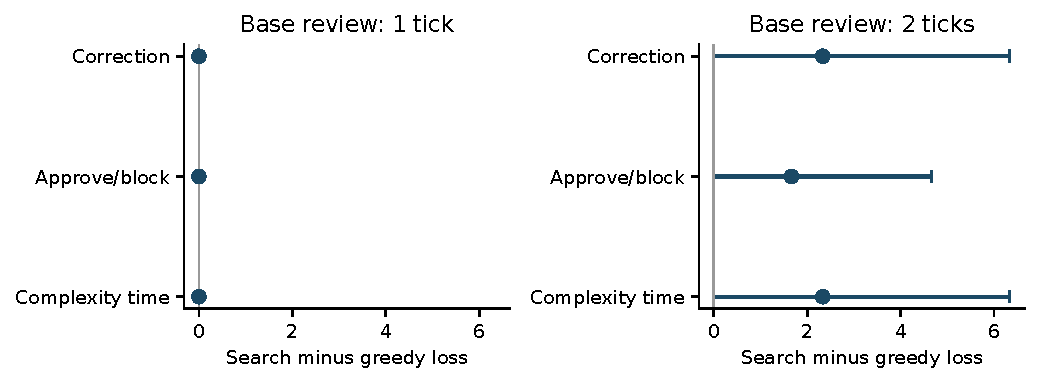
\includegraphics[width=0.98\textwidth]{../artifacts/stage6_robustness/analysis/fresh/figures/paired_loss.pdf}

\caption{Fresh operational sensitivity. Points are search minus greedy mean loss; bars are 95\% paired bundle-bootstrap intervals. Only approve/block at base duration two is primary. Degenerate one-tick intervals describe ties in this sample, not population equivalence.}

\label{fig:robustness}\end{figure*}

\subsection{Scheduling Mechanism and Error Ranking}

Search and greedy review sequences differ in six of 24 fresh runs at base duration two, versus one search--EDF difference. On search's states, 19 dispatches have multiple eligible requests and six have different greedy/search heads. These are repeated states for descriptive analysis, not additional independent observations.

The first unfavorable example is bundle 06, replicate 2. At tick zero, search reviews a correct cancellation with cutoff two, planning to preserve both currently available opportunities. Greedy instead blocks the wrong modification by tick two. A correct exchange arrives at tick one. When search becomes free, its frozen estimate prioritizes that exchange, and the modification posts at tick five. Search loss is eight versus greedy's four. The primary example rule finds no fresh search benefit. The first tie contains a blocked incomplete return and an unstaged modification, giving equal loss eight.

The frozen estimator's aggregate Brier score is 0.17144, versus 0.17998 for its pooled estimate; AUROC is 0.6581. Yet modification has eight errors among 13 staged proposals, versus four among 18 returns/exchanges, while predicted risks rank those families in the opposite order. All 20 staged cancellations are correct. This retrospective evidence helps explain the unfavorable trace without granting labels to the scheduler or refitting on evaluation data. Eight source cases produce different proposals across the three replicates, and four have mixed initial correctness.

\subsection{Saved-Preparation Sensitivity}

The separate post hoc analysis replays all 1,152 original reference traces exactly and adds the declared variants on the same 288 preparations. At base duration two, restricted-authority search minus greedy is $+0.125\;[-0.167,0.500]$, with one win, 29 ties and two losses. Complexity time gives $+0.500\;[-0.083,1.250]$, with one win, 28 ties and three losses. These results do not replace the original $+0.250$ primary comparison. Blocking changes search's actual sequence in only two of 96 runs relative to correction. The first saved-data benefit remains available as a trace alongside the fresh null and unfavorable examples.


\section{DISCUSSION}
\noindent Planning helps when valuable interventions compete for time and ordering preserves opportunities that greedy selection would lose. Constructed maintenance competition provides that condition. The original maintenance workload and the retail study show why a favorable mechanism does not imply a general policy ranking. Public contention can involve correct requests, some errors are already infeasible, and later arrivals are outside the planner's current state.\draftcredit

Capacity changes the opportunity set. When every useful queued error can be corrected, simple review policies can match search despite different orders. When capacity is severely constrained, too few feasible combinations may remain for ordering to help. More completed reviews can then coexist with fewer corrections. The meaningful outcome is preventable operational consequence, not sequence diversity alone.

The reviewer objective and authority must also be explicit. A search policy that optimizes weighted cost can close fewer jobs correctly. A block-only reviewer can prevent processing harm while leaving service unfinished. These outcomes are consistent with their objectives and should not be converted into claims of universal superiority. The robustness study isolates these mechanisms without changing risk estimates or agent preparation.

Our evidence is limited to one model, bounded workloads and perfect diagnosis. Synthetic fault generation gives a transparent observation model, while public retail source cases offer genuine tools but shared templates and possible training exposure. Scripted confirmation and complete-transaction correction simplify customer interaction. Deadlines, processing weights and complexity times are constructed quantities. Exact annotated equality can overstate some operational distinctions. No measured human review performance, retailer savings or large-queue scalability follows.

\section{CONCLUSION}
\noindent Shared review can be studied as a timed intervention problem with an application-specific preventable-loss function. The resulting framework exposes differences between uncertainty, urgency, expected benefit and queue planning while preserving the information boundary. Frozen maintenance evidence supports a conditional planning benefit and objective tradeoffs. The retail primary result is unfavorable to search, and its operational follow-up tests what changes when review can block rather than complete a transaction. The combined evidence supports analyzing capacity, error ranking and corrective authority together when designing oversight for language model workflows.\draftcredit

\section*{AI ASSISTANCE AND REPRODUCIBILITY}
OpenAI Codex assisted implementation, test and analysis code, source checking, figure code, and drafting and revision throughout this manuscript and supplement \cite{openai2026codex}. Numerical results derive from logged GPU generations and deterministic simulation, with declared tests and replay checks. Figures plot those saved measurements. AI is not an author. Human authors remain responsible for verification, interpretation and submission. Source snapshots, declarations, raw evidence, ledgers and reproduction commands accompany the local research package. Previously disclosed publication redactions remove unsolicited credential-like model text from auxiliary arguments and prompt histories, preserving original hashes and unchanged transactions, labels and outcomes. Exact originals remain on the authorized pod. Deterministic replay does not promise bitwise regeneration from a seed.

\balance
\bibliographystyle{apalike}
{\small\bibliography{references}}
\end{document}
